\documentclass[../main.tex]{subfiles}

\begin{document}
	\section{Transfer of Thermal Energy}
	\begin{preamb}
		Heat can be transferred in multiple ways. In this chapter we will look at three different methods for heat transfer.
	\end{preamb}	
	
	Heat always flows from a region of higher temperature to a region of lower temperature. Net flow of thermal energy occurs only when there is a difference in temperature.
	
	\begin{center}
		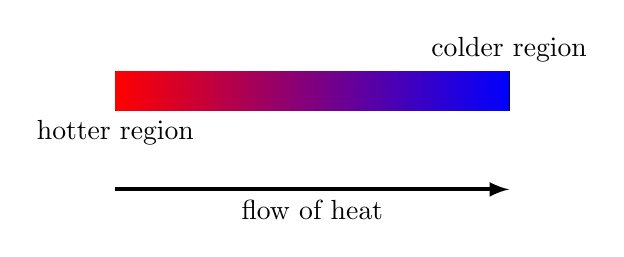
\begin{tikzpicture}
			\draw (0,0) [anchor=north] node {hotter region} rectangle (5,0.5) node [anchor=south] {colder region};
			\shade [left color=red, right color=blue] (0,0) rectangle (5,0.5);
			\draw [line width=0.5mm, -latex] (0,-1) -- (5,-1) node [pos=0.5, anchor=north] {flow of heat};
		\end{tikzpicture}
	\end{center}
	
	\pdef{Conduction}{Conduction is the process whereby particles within a medium without the movement of the medium itself.}
	
	Particles collide with neighbouring particles and that energy gets transferred down the entire object, causing the object to increase in temperature.
	
	Metals can conduct heat better due to \textbf{electron diffusion}.
	
	\pdef{Convection}{Convection is the transfer of thermal energy by means of convection currents in a fluid due to a difference in density.}
	
	
	\pdef{Radiation}{Radiation is the transfer of thermal energy in the form of electromagnetic waves such as infrared radiation without the aid of a medium.}
	Factors that affect the rate of radiation include:
	\begin{itemize}
		\item \textbf{Colour:} darker objects radiate heat better than lighter objects (see emissivity)
		\item \textbf{Surface:} rougher surfaces radiate heat better than smoother surfaces (due to higher surface area)
	\end{itemize}
	
	Further reading: Radiation is modelled by the Stefan-Boltzmann Law:
		\[ P = A \varepsilon \sigma T^4 \]
	where \(\varepsilon\) is the emissivity and \(\sigma\) is the Stefan-Boltzmann constant, \SI{5.67e-8}{\watt \, \meter^{-2} \, \kelvin^{-4}}.
\end{document}
